\chapter{Graph Attention Networks Embedded Knowledge Tracing Model With Transformer}

% **************************** Define Graphics Path **************************
\ifpdf
    \graphicspath{{Chapter3/Figs/Raster/}{Chapter3/Figs/PDF/}{Chapter3/Figs/}}
\else
    \graphicspath{{Chapter3/Figs/Vector/}{Chapter3/Figs/}}
\fi

\section{Motivation}
%本章节为该推荐系统的一个核心部分,即通过知识追踪的方式获取学生的知识掌握状态。知识追踪是根据学生的以往的答题记录来建模学生的知识掌握情况,从而获取学生的知识状态。知识追踪的模型非常丰富,早期的知识追踪模型一般基于一阶马尔可夫模型的贝叶斯知识追踪(BKT),它们的基础假设是学生答题基于一系列知识点,这些知识点之间被认为是相互不相关的,因此它们之间是独立表示,这种做法无法捕捉不同概念之间的关系也无法表征复杂的概念转换。在2015年,Piech等人提出了深度知识追踪模型(DKT),首次将长短期记忆网络(LSTM)应用于知识追踪任务,它无需进行知识点标注,而是包含一个知识的隐含状态,当时取得了超过BKT的基线性能,它标志着基于神经网络模型的知识追踪研究的序幕。但DKT无法输出知识的隐藏状态,可解释性不足。而且DKT用将所有记忆存储于一个隐藏向量中,对于长序列的预测性能不够理想。针对这个问题,记忆增强网络(MANN)被提出来,它允许网络保留多个隐藏状态向量,并分别读写这些向量。在2017年,张等人提出了Dynamic Key-Value Memory Networks(DKVMN),它参考了MANN的设计,针对知识追踪任务进行了优化,优化了MANN对于知识追踪任务的输入输出不同域的问题。DKVMN采用了键值对作为存储器结构,能避免过拟合、参数少,以及通过潜在概念自动发现相似练习,取得了相对BKT和DKT更好的预测性能。同时该模型也具有较好的可解释性,它将问题相关潜在概念存储于键矩阵中,对概念掌握程度存储于值矩阵中,通过对输入练习与键矩阵的相关性对值矩阵进行更新。但这些模型仍存在长依赖的问题。为了解决这个问题,设计了一个hop-LSTM结构来聚合相似的习题的隐藏状态的Sequential Key-Value Memory Networks(SKVMN)被提出来。但现有的模型往往对于知识点之间的高阶连接考虑不足,或者简单地将知识点作为相互独立的节点,或者将知识点作为简单的层次模型,但实际上,知识点之间是高阶的图状结构,在这种情况下,采用图神经网络来表征知识点之间的关系,训练问题embedding和概念embedding是更好的选择,因此在本章,我们提出了基于图神经网络的知识追踪模型,它利用高阶问题-知识点关系,来解决稀疏性和复杂知识点依赖问题,同时,它通过问题日志模块,可以学习学生的掌握速度,从而更好表征知识追踪过程。

This section is a core part of this recommendation system, which is to obtain the student's knowledge mastery status by means of knowledge tracing. knowledge tracing is to model students' knowledge mastery based on their past answer records to obtain students' knowledge status. knowledge tracing models are abundant, and early knowledge tracing models are generally based on the Bayesian knowledge tracing (BKT)\cite{yudelson2013individualized} of first-order Markov models, which are based on the assumption that student answers are based on a series of knowledge points that are considered to be unrelated to each other and therefore represented independently of each other, an approach that cannot capture the relationships between different concepts nor characterize complex conceptual transformations. In 2015, Piech et al. proposed the Deep knowledge tracing Model (DKT)\cite{piech2015deep}, the first application of a long short-term memory network (LSTM) to the knowledge tracing task, which does not require knowledge point annotation but contains an implicit state of knowledge, achieving a baseline performance over BKT at that time, and it marked the prologue of knowledge tracing research based on neural network models. However, DKT could not output the hidden state of knowledge, and the interpretability was insufficient. Moreover, DKT used to store all memories in a hidden vector, and the prediction performance was not satisfactory for long sequences. To address this problem, Memory Augmented Neural Network (MANN)\cite{santoro2016meta} was proposed, which allows the network to keep multiple hidden state vectors and read and write these vectors separately. In 2017, Zhang et al. proposed Dynamic Key-Value Memory Networks (DKVMN)\cite{zhang2017dynamic}, which refers to the design of MANN for knowledge tracing tasks and optimizes MANN for knowledge tracing tasks with different input and output domains. DKVMN uses key-value pairs as the memory structure, which can avoid over better prediction performance relative to BKT and DKT is achieved by using key-value pairs as the memory structure, which can avoid overfitting, fewer parameters, and automatic discovery of similar exercises through latent concepts. The model also has better interpretability, as it stores the problem-related potential concepts in the key matrix and the mastery of the concepts in the value matrix, and updates the value matrix by correlating the input exercises with the key matrix. However, these models still suffer from the problem of long dependencies. To solve this problem, Sequential Key-Value Memory Networks (SKVMN)\cite{Abdelrahman_2019}, which designs a hop-LSTM structure to aggregate the hidden states of similar exercises, was proposed. However, existing models often do not consider enough the higher-order connections between knowledge points, or simply treat knowledge points as mutually independent nodes, or treat knowledge points as simple hierarchical models, but in fact, knowledge points are higher-order graph-like structures, in which case, using graph neural networks to characterize the relationships between knowledge points, training problem embedding and concept embedding is a better choice, so in this chapter, we propose a graph neural network-based knowledge tracing model, which uses higher-order problem-knowledge point relationships to solve the sparsity and complex knowledge point dependency problems, and at the same time, it can learn the mastery speed of students through the problem logging module, so as to better characterize the knowledge tracing process.

\section{Related Theory}
\subsection{Knowledge Tracing}
%知识追踪为智能化和自适应教育提供了条件,它具有个性化和自动化的特点。知识追踪任务从学生的历史学习记录来追踪学生的知识状态变化,预测未来的学习表现,从而针对性地给予学习辅导。其本质基于学生的过去的学习表现来获取当前的学习状态,从而预测将来的学习表现。其实际做法是,对学生过去的答题记录进行数据分析和过程建模,从而建模当前的学生学习状态数据,让模型跟做学生的每个阶段的学习状态,并基于学习状态数据来预测习题答对的概率。在学科学习中,学科知识由一系列知识点组成,学生的学习状态实际上基于对于各个知识点的掌握情况。而知识追踪一般的形式为给定一个学生的答题序列,该序列由一系列习题构成,习题又与特定的知识点相关联,在知识追踪中的一个基本假设是,学生的答题表现基于对知识点的掌握。而学生的答题表现即可用于反推学生对于各个知识点的掌握情况,即学习状态的掌握情况。

%知识追踪任务的数学表示为一个学生在一个习题序列上的交互式答题记录$X_t=(x_1,x_2,⋯,x_t)$,根据该记录通过建模来获取学生的学习状态,并预测学生在下一次练习中的表现$x_{t+1}$。其中$x_t$通常表示为一个有序对$(q_t,a_t)$,有序对表示学生在时间$t$回答了问题$q_t$,$a_t$表示问题的得分情况,也有许多知识追踪任务用答对或答错来表示,此时$a_t$为0或者1,在此情况下,实际上预测的是对于下一个问题回答正确的概率$P(a_{t+1}=1|a_t)$。如图ref{kt1}。


Knowledge tracing provides the conditions for intelligent and adaptive education, which is personalized and automated. Knowledge tracing tasks track changes in students' knowledge status from their historical learning records, predict future learning performance, and provide targeted learning coaching. The essence is to obtain the current learning status based on the student's past learning performance to predict the future learning performance. The actual practice is to analyze the data and process modeling of students' past answer records, so as to model the current student learning status data, and let the model follow the learning status of students at each stage, and predict the probability of correct answers to the exercises based on the learning status data. In subject learning, subject knowledge consists of a series of knowledge points, and students' learning status is actually based on their mastery of each knowledge point. The general form of knowledge tracing is that given a sequence of student answers, which consists of a series of exercises associated with a specific knowledge point, a basic assumption in knowledge tracing is that student performance is based on mastery of the knowledge point. The student's performance can be used to infer the student's mastery of each knowledge point, i.e., the mastery of the learning state.

The mathematical representation of the knowledge tracing task is an interactive answer record $X_t=(x_1,x_2,⋯,x_t)$ of a student on an exercise sequence, based on which the student's learning status is obtained by modeling and predicting the student's performance in the next exercise $x_{t+1}$. Where $x_t$ is usually represented as an ordered pair $(q_t,a_t)$, the ordered pair indicates that the student answered the question $q_t$ at time $t$, and $a_t$ indicates the score of the question, also many knowledge tracing tasks are represented by correct or incorrect answers, when $a_t$ is 0 or 1. In this case, what is actually predicted is the probability of answering correctly for the next question $P(a_{t+1}=1|a_t,a_{t-1},...,a_1)$. As shown in the figure \ref{kt1}.

\subsection{Graph Neural Networks}
%在提取欧氏空间数据特征方面取得了较大成功的传统神经网络模型,在非欧氏空间上的应用却效果并不理想。而目前,许多实际的应用场景正式非欧式空间生成的。在知识追踪过程中,知识点之间的联系正是一种非欧式空间的结构,即知识图结构。图的不规则性和复杂性对于传统的深度学习算法提出了巨大的挑战,图的节点的联系的可变性导致了庞大的计算量,这使得一些在欧氏空间表现良好的传统神经网络模型无法直接应用于非欧式空间。例如,在处理图像中,图像的每个像素都是相互独立的,卷积神经网络对于图像这种稳定单一且个部分相互独立的结构较为容易计算和并行化,但对于每个节点都与其他节点联系并有依赖关系的图结构来说,情况并非如此。为了表征图节点之间相互依赖的关系,图神经网络(GNN)被提出来。 GCN作为图神经网络的开山之作,将图像处理中的卷积操作简单的用到图结构数据处理中来,并且给出了具体的推导。它实际上是聚合图邻居节点的特征做一个线性变换。为了能够解决图传播深度不足的问题,还可以堆叠多层GCN层以捕捉k-hop的邻居节点信息。GCN通过对于图的结构的编码取得了优秀的节点表征性能。但GCN的处理方式需要将整个图放到计算显存内,这限制了其计算性能。且它需要预先输入图的结构信息,这限制了它的应用。为了解决GCN聚合邻居节点忽略不同邻居节点的权重不同的问题, Graph Attention Networks(GAT) 引入了masked self-attention机制,计算每个节点的表示时,根据邻居节点特征来分配不同权值。它无需使用预先构建好的图,因此只需要知道邻居节点即可,这大大增加了计算速度。

%图嵌入是一个图神经网络的重要研究课题,它通过保留图的网络拓扑结构和节点信息,将图中节点表示为低维向量,然后通过其他的机器学习算法进行处理。在本章中,我们通过一个图嵌入算法来表征知识点之间的关联和知识点信息,从而获取对于知识结构的嵌入学习。

The traditional neural network model, which has achieved greater success in extracting features from Euclidean space data, has not worked well for applications on non-Euclidean spaces. And currently, many practical application scenarios are formally generated in non-Euclidean spaces. In the process of knowledge tracing, the connection between knowledge points is exactly a structure of non-Euclidean space, i.e., knowledge graph structure. The irregularity and complexity of graphs pose a great challenge to traditional deep learning algorithms, and the variability of the connections of the nodes of graphs leads to a huge computational effort, which makes some traditional neural network models that perform well in Euclidean space cannot be directly applied to non-Euclidean space. For example, in processing images where each pixel of the image is independent of each other, convolutional neural networks are easier to compute and parallelize for structures like images that are stable and single and have individual parts independent of each other, but this is not the case for graph structures where each node is connected to and has dependencies on other nodes. To characterize the interdependencies between graph nodes, Graph Neural Networks (GNNs) are proposed. 

There are five major classes of graph neural networks: Graph Convolution Networks (GCN), Graph Attention Networks(GAN), Graph Autoencoders(GAE), Graph Generative Networks(GGN), and Graph Spatial-temporal Networks(GSN). GCN, the pioneer of graph neural networks, simply applies the convolution operation in image processing to graph structured data processing and gives a specific derivation. It actually aggregates the features of graph neighbor nodes to make a linear transformation. To solve the problem of insufficient depth of graph propagation, multiple GCN layers can be stacked to capture the k-hop neighbor node information. However, the GCN processing requires putting the whole graph into the computational memory, which limits its computational performance. It also requires pre-inputting the graph structure information, which limits its application. To solve the problem that GCN aggregates neighbor nodes ignoring different weights of different neighbor nodes, Graph Attention Networks (GAT) introduces a masked self-attention mechanism to compute the representation of each node by assigning different weights according to the neighbor node characteristics. It does not need to use a pre-constructed graph, so only the neighbor nodes need to be known, which greatly increases the computational speed.

Graph embedding is an important research topic in graph neural networks, which represents nodes in a graph as low-dimensional vectors by preserving the network topology and node information of the graph, which is then processed by other machine learning algorithms. In this chapter, we characterize the association between knowledge points and knowledge point information by a graph embedding algorithm to obtain the learning of embedding for knowledge structures. 

\subsection{Transformer}


\section{Proposed Model}

\subsection{Algorithm Overview}
%本节的关键点是对学生的知识追踪,本文提出了一种基于图自注意力网络和Transformer模型的知识追踪模型GATKT。在实验验证阶段,该模型在几个数据集上的基线性能达到了SOA。本模型的第一层为embedding聚合层,该层用一个GAT来聚合问题embedding和知识点embedding,并展示问题和知识点的内在联系,它可以解决数据稀疏性问题和知识点依赖和复杂关系问题。第二层为一个Transformer-based知识追踪模型,该层参考Google提出的著名的Transformer模型 \cite{vaswani2017attention},设计了一个基于Transformer机制的知识追踪模型,它输入问题和技能embedding,输出对于下一个问题的答对的预测。通过这种机制,该模型可以实现对long-range的依赖的学习。此外,本模型可以通过解码器来输出隐藏的知识状态,这是下一阶段进行习题推荐的关键。总而言之,该模型的总体架构图可以见图\ref{},并分为以下几个模块。
%1. 基于GAT的embedding层:该层用embedding方法来表征问题,知识点和回答。在该图神经网络中,每个问题代表一个节点,它与若干知识点节点连接,这些知识点节点再与与之相关的问题节点连接。而问题与问题不直接连接,考虑到知识点的相关性,知识点与知识点可以直接连接。其结构如图\ref{}。这个embedding层不进行预训练,而是与其他层进行总体训练来优化最终结果。
%2. 问题与知识点关系图:该图表征问题与相关联的知识点,问题与问题之间不直接相连,而知识点可以与若干问题或知识点相连。
%3. 基于Transformer的知识追踪层:该层类似传统Transformer结构,具有encoder和decoder两部分,它学习关联知识点和问题的权值矩阵,可以解决知识点依赖问题。通过注意力机制,它也可以capture关联知识点相似的问题。


The key point of this section is to track students' knowledge. This paper proposes a knowledge tracking model based on graph self attention network and Transformer model GATKT. In the experimental verification phase, the baseline performance of the model on several datasets achieves SOA. The first layer of this model is the embedding aggregation layer. In this layer, a gat is used to aggregate the problem embedding and the knowledge point embedding, and to show the internal relationship between the problem and the knowledge point. It can solve the problem of data sparsity and the problem of knowledge point dependence and complex relationship. The second layer is a transformer based knowledge tracking model. Referring to the famous transformer model proposed by Google Brain \cite{vaswani2017attention}, this layer designs a knowledge tracking model based on the transformer mechanism, which inputs questions and skills embedding, and outputs the prediction of the correct answer to the next question. Through this mechanism, the model can realize the learning of long range dependence. In addition, the model can output the hidden knowledge state through the decoder, which is the key to exercise recommendation in the next stage. In a word, the overall architecture diagram of the model can be seen in Figure \ref{fig1}, which is divided into the following modules:
\begin{enumerate}
  \item GAT-based embedding layer: embedding layer based on gat: this layer uses embedding method to represent questions, knowledge points and answers. In the graph neural network, each problem represents a node, which is connected with several knowledge nodes, and these knowledge nodes are connected with the related problem nodes. Considering the relevance of knowledge points, knowledge points and knowledge points can be directly connected. The structure is shown in the figure \ref{fig2}. This embedding layer does not carry out pre training, but carries out overall training with other layers to optimize the final result.
  \item GAT-based knowledge state tracking layer: this layer establishes a graph of knowledge points, which is used to track the students' mastery of knowledge points. This layer updates the knowledge state through the knowledge state, and finally it will be used in the subsequent recommendation process.
  \item Knowledge tracing layer based on Transformer: this layer is similar to the traditional transformer structure, and has two parts: encoder and decoder. It learns the weight matrix of knowledge points and problems, and can solve the problem of knowledge point dependence. Through the attention mechanism, it can also capture similar problems of knowledge points.
\end{enumerate}

\begin{figure}[h]
	\centering
	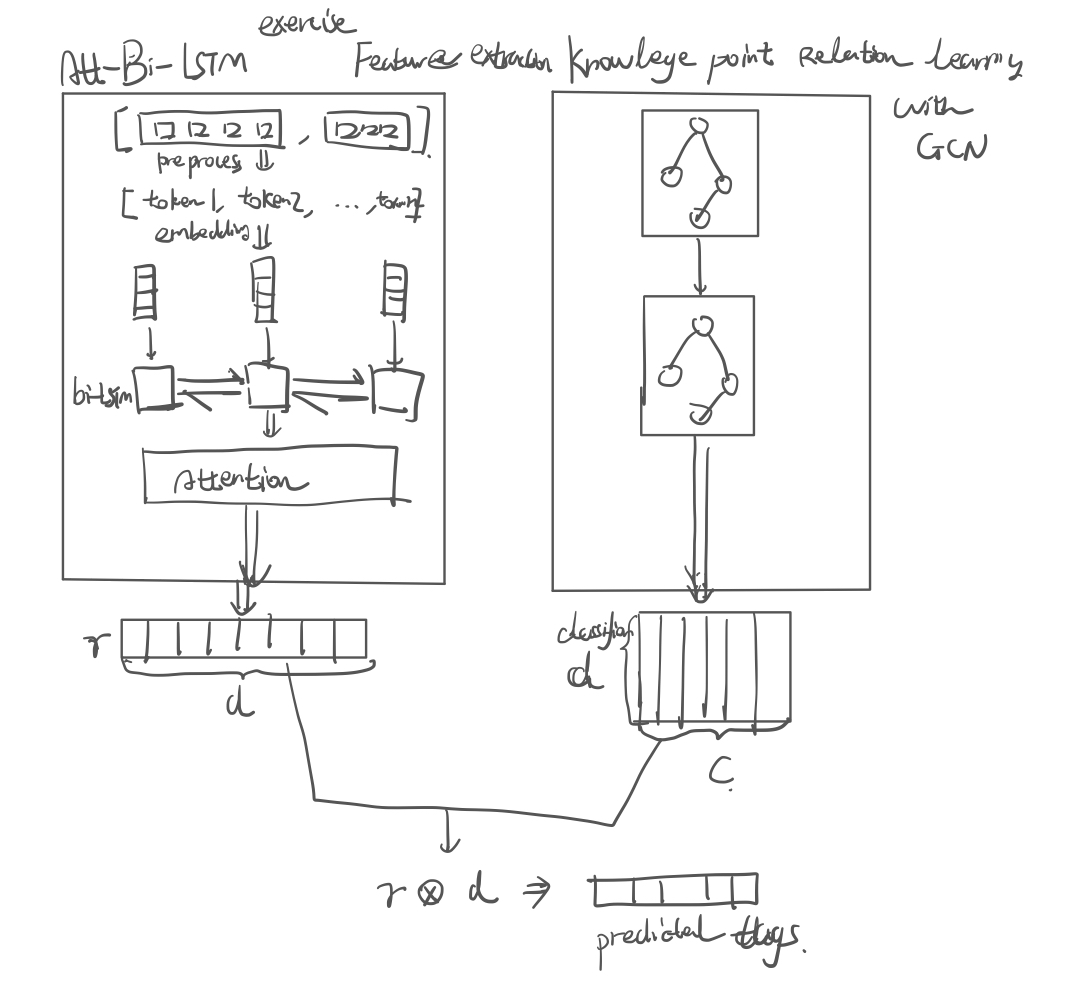
\includegraphics[width=1.0\textwidth]{ch2-fig1.jpeg}
	\caption{Overview Model Structure}
	\label{fig1}
\end{figure}
\begin{figure}[h]
	\centering
	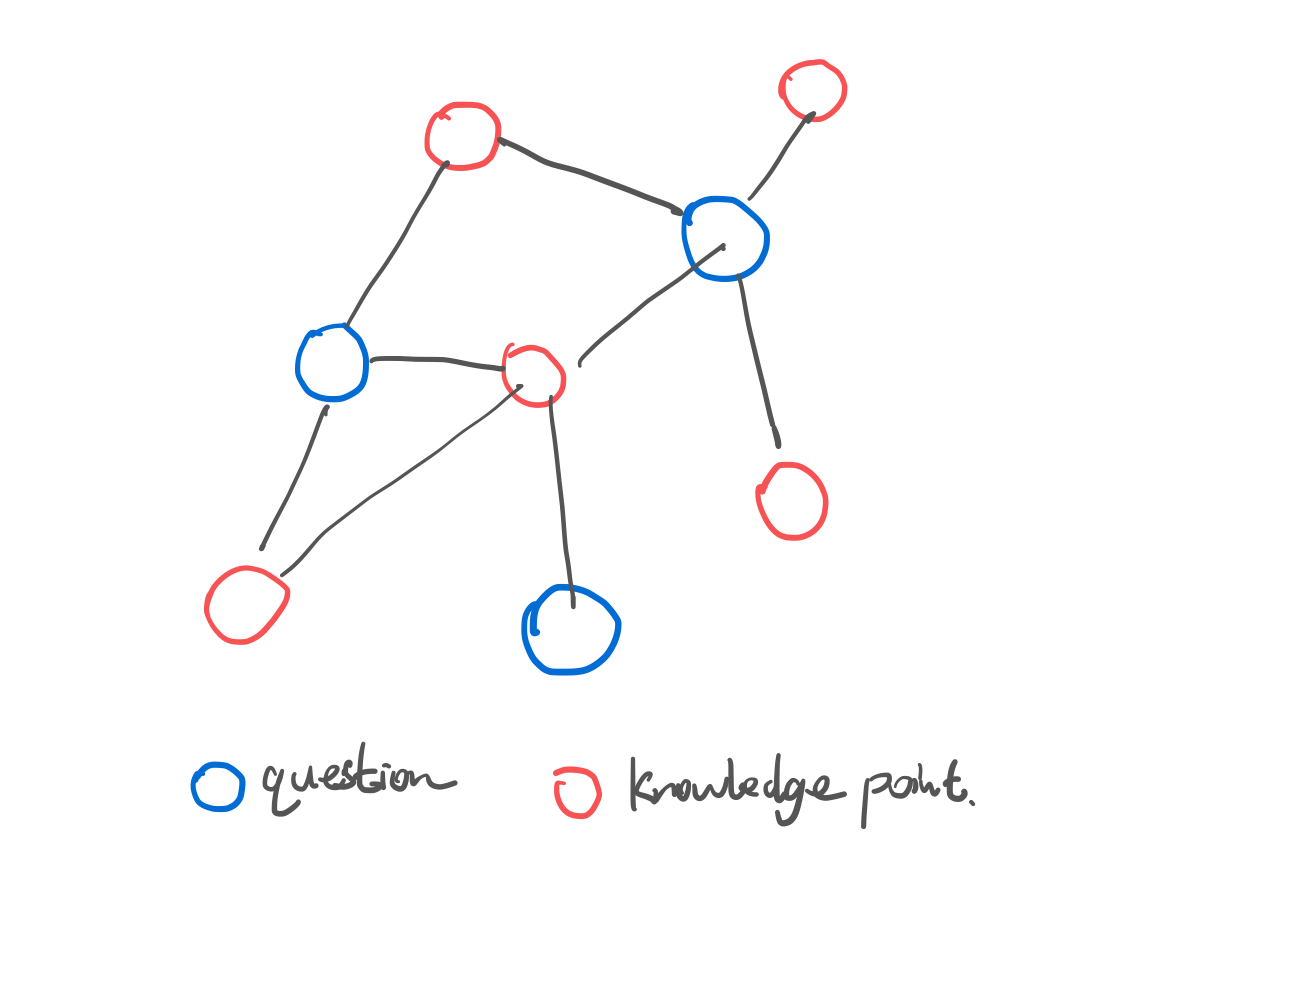
\includegraphics[width=1.0\textwidth]{ch2-fig2.jpeg}
	\caption{The Graph of Knowledge Point and Question}
	\label{fig2}
\end{figure}


\subsection{GAT-based Embedding Layer}
%本节中,采用了图自注意力网络来对问题-知识点关联图进行embedding。它用于降低表征问题数据中知识点的数据稀疏性。我们把第i个问题记作$q_i$,学生对第i个问题的回答记作$a_i$,其中$a_i\in\{0,1\}$,则答题记录记为$X=\{x_1,x_2,...x_{t-1}\}$,其中$x_i=(q_i,a_i)$,我们基于前$t-1$次的答题记录来预测第$t$题的回答正确概率。对于每个问题$q_i$,有一系列的知识点与之相关,这些知识点记作$\{p_1,p_2,...,p_{n_i}\}$。在这里进行embedding计算可以获取问题之间的深层次关联关系,即知识点的相关性。用图结构可以较为理想地做到这一点。从直观上来说,也可以通过对于知识点的掌握情况来推知问题的答对概率。该方法也可以建立对于问题-知识点的更好的表征。

In this section, the graph self attention network is used to embed the problem knowledge point association graph. The embedding method can reduce the sparsity in representing the knowledge points in question data. Let's denoted the i-th question as $q_i$. The answer to question I is $a_i$. The answer record is $x = \{x_1,x_2,...x_{T-1}\}$, where $X_i=(q_i,a_i)$. Based on the answer records of the previous $t-1$ times, we predict the correct probability of the answer to question $t$. For each question $q_i$, there are a series of knowledge points related to it, these knowledge points are denoted as $\{p_1,p_2,...,p_{n_i}\}$, $n_i$ marks the number of knowledge points related to the question $q_i$. Similarly, a knowledge point $p_j$ has also several related question $q_1,...,q_{n_j}$, where $n_j$ is the number of question related to the knowledge point $p_j$. So a graph $\mathcal{G}$ can be used to represent the relation of question-knowledge point, where $\mathcal{G}=\{(q, r_{qp}, p) | q \in \mathcal{Q}, s \in \mathcal{S}}$ and $\mathcal{Q}$ denotes question sets and $\mathcal{P}$ denotes knowledge point sets respectively. $r_{qp}=1$ if $q$ is related to $p$. 

In this part, embedding calculation can obtain the deep correlation between problems, that is, the correlation of knowledge points. This can be achieved with graph structure. Intuitively speaking, we can also infer the correct answer probability of the question by mastering the knowledge points. This method can also establish a better representation of problem knowledge points. In the question-knowledge graph, GAT can capture the high order relation for n-hop neighboring nodes. Also, GAT uses the idea of transformer for reference and introduces masked self attention mechanism. When calculating the representation of each node in the graph, it will assign different weights to its neighbors according to their different characteristics. 

GAT applies an attention mechanism to weighted summation of neighboring node features. The weights of the neighboring node features depend entirely on the node features and are independent of the graph structure. In GAT, each node in the graph can be assigned different weights to neighboring nodes based on their characteristics. With the introduction of the attention mechanism, it is only relevant to adjacent nodes, i.e., nodes that share edges, without the need to get information about the whole graph. Specifically, the node of GAT network represents the knowledge point embedding or question embedding. Denote the node as $i$ and the neighbor node set as $\mathcal{N}_{i}$ and the embedding of node as $x_i$, the input of the graph attention layer is $x=\left\{\overrightarrow{x_{1}}, \overrightarrow{x_{2}}, \overrightarrow{x_{3}} \ldots \overrightarrow{x_{n}}|\overrightarrow{x_{i}}\in \mathbb{R}_{F}\right\}$ and the output is $ x=\left\{\overrightarrow{x_{1}}^{\prime}, \overrightarrow{x_{2}}^{\prime}, \overrightarrow{x_{3}}^{\prime} \ldots \overrightarrow{x_{n}}^{\prime}|\overrightarrow{x_{i}}^\prime\in \mathbb{R}_{F^\prime}\right\}$, where $n$ is the number of nodes and $F$ is the number of node features. represents the features of all nodes, and $F^{\prime}$ denotes the output node features. In order to get the corresponding input and output transformations, we need to perform at least one linear transformation based on the input features to get the output features, so we need to train a weight matrix for all nodes: $W \in \mathbb { R } ^ { F ^ { \prime } \times F }$, and this weight matrix is the relationship between the F features of the input and the F′ features of the output.

To achieve better high dimension feature representation, we need at least one linear transformation from low-dimensional to high-dimensional features. Therefore, a linear transformation is first done for the node features and then the coefficients are calculated. The attention mechanism of self-attention is implemented for each node, and the attention coefficients (Attention coefficients) and its softmax value are:
$$e_{i j}=a\left(\mathbf{W} \vec{x}_{i}, \mathbf{W} \vec{x}_{j}\right)$$
$$\alpha_{i j}=\operatorname{softmax}_{j}\left(e_{i j}\right)=\frac{\exp \left(e_{i j}\right)}{\sum_{k \in \mathcal{N}_{i}} \exp \left(e_{i k}\right)}$$

The $e_{ij}$ and $\alpha_{ij}$ represents the importance of node $i$ to node $j$. 

In General, the complete attention mechanism is:
$$
\alpha_{i j}=\frac{\exp \left(\text{LeakyReLu}\left(\overrightarrow{\mathrm{a}}^{T}\left[W \vec{h}_{i} \| W \vec{h}_{j}\right]\right)\right)}{\sum_{k \in N_{i}} \exp \left(\text{LeakyReLu}\left(\overrightarrow{\mathrm{a}}^{T}\left[W \vec{h}_{i} \| W \vec{h}_{k}\right]\right)\right)}
$$, where $||$ means concatenation operation. It is a single-layer feedforward neural network, $\overrightarrow { \mathrm { a } } \in \mathbb { R } ^ { 2 F ^ { \prime } }$ is the weight matrix connecting the layers in the neural network, and a LeakyReLu function is also added to the output layer of this feedforward neural network. The procedure is like Figure \ref{fig3};

\begin{figure}[h]
	\centering
	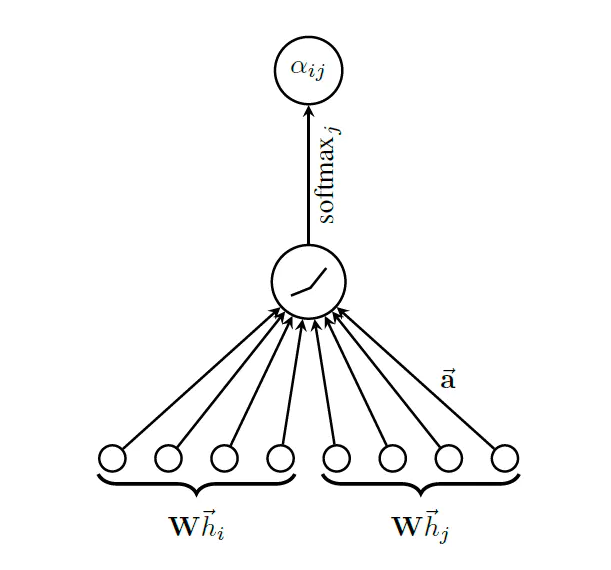
\includegraphics[width=1.0\textwidth]{ch2-fig3.png}
	\caption{Feature extraction and attention mechanism}
	\label{fig3}
\end{figure}

Here, since the graph structure information is to be considered, the concept of masked attention is introduced, which means that the denominator of the softmax considers only the first-order information about the neighbors. By this method, each node then gets a weight about the neighboring nodes and then the combined representation of the nodes is obtained by summing.

$$\vec{x}_{i}^{\prime}=\sigma\left(\sum_{j \in \mathcal{N}_{i}} \alpha_{i j} \mathbf{W} \vec{x}_{j}\right)$$
where $\sigma$ are the non-linear transformation such as ReLU or LeakyReLU. If the edge $j \to i$ does not exist, we can simply omit the calculation of $\alpha_{ij}$, which can reduce the calculation. The formula means that the output characteristics of this node are related to all the nodes adjacent to it and are obtained after the nonlinear activation of their linear sum.

To make the result of self-attention more stable. The multi-headed attention mechanism can be used here, like Figure \ref{fig4}. Multi-head attention is actually a combination of multiple self-attention structures, each head learns features in a different representation space, and multiple heads may learn slightly different attention focus, which gives the model more capacity.
$K$ independent attention mechanisms can be achieved by connecting $k$ features together.
\begin{figure}[h]
	\centering
	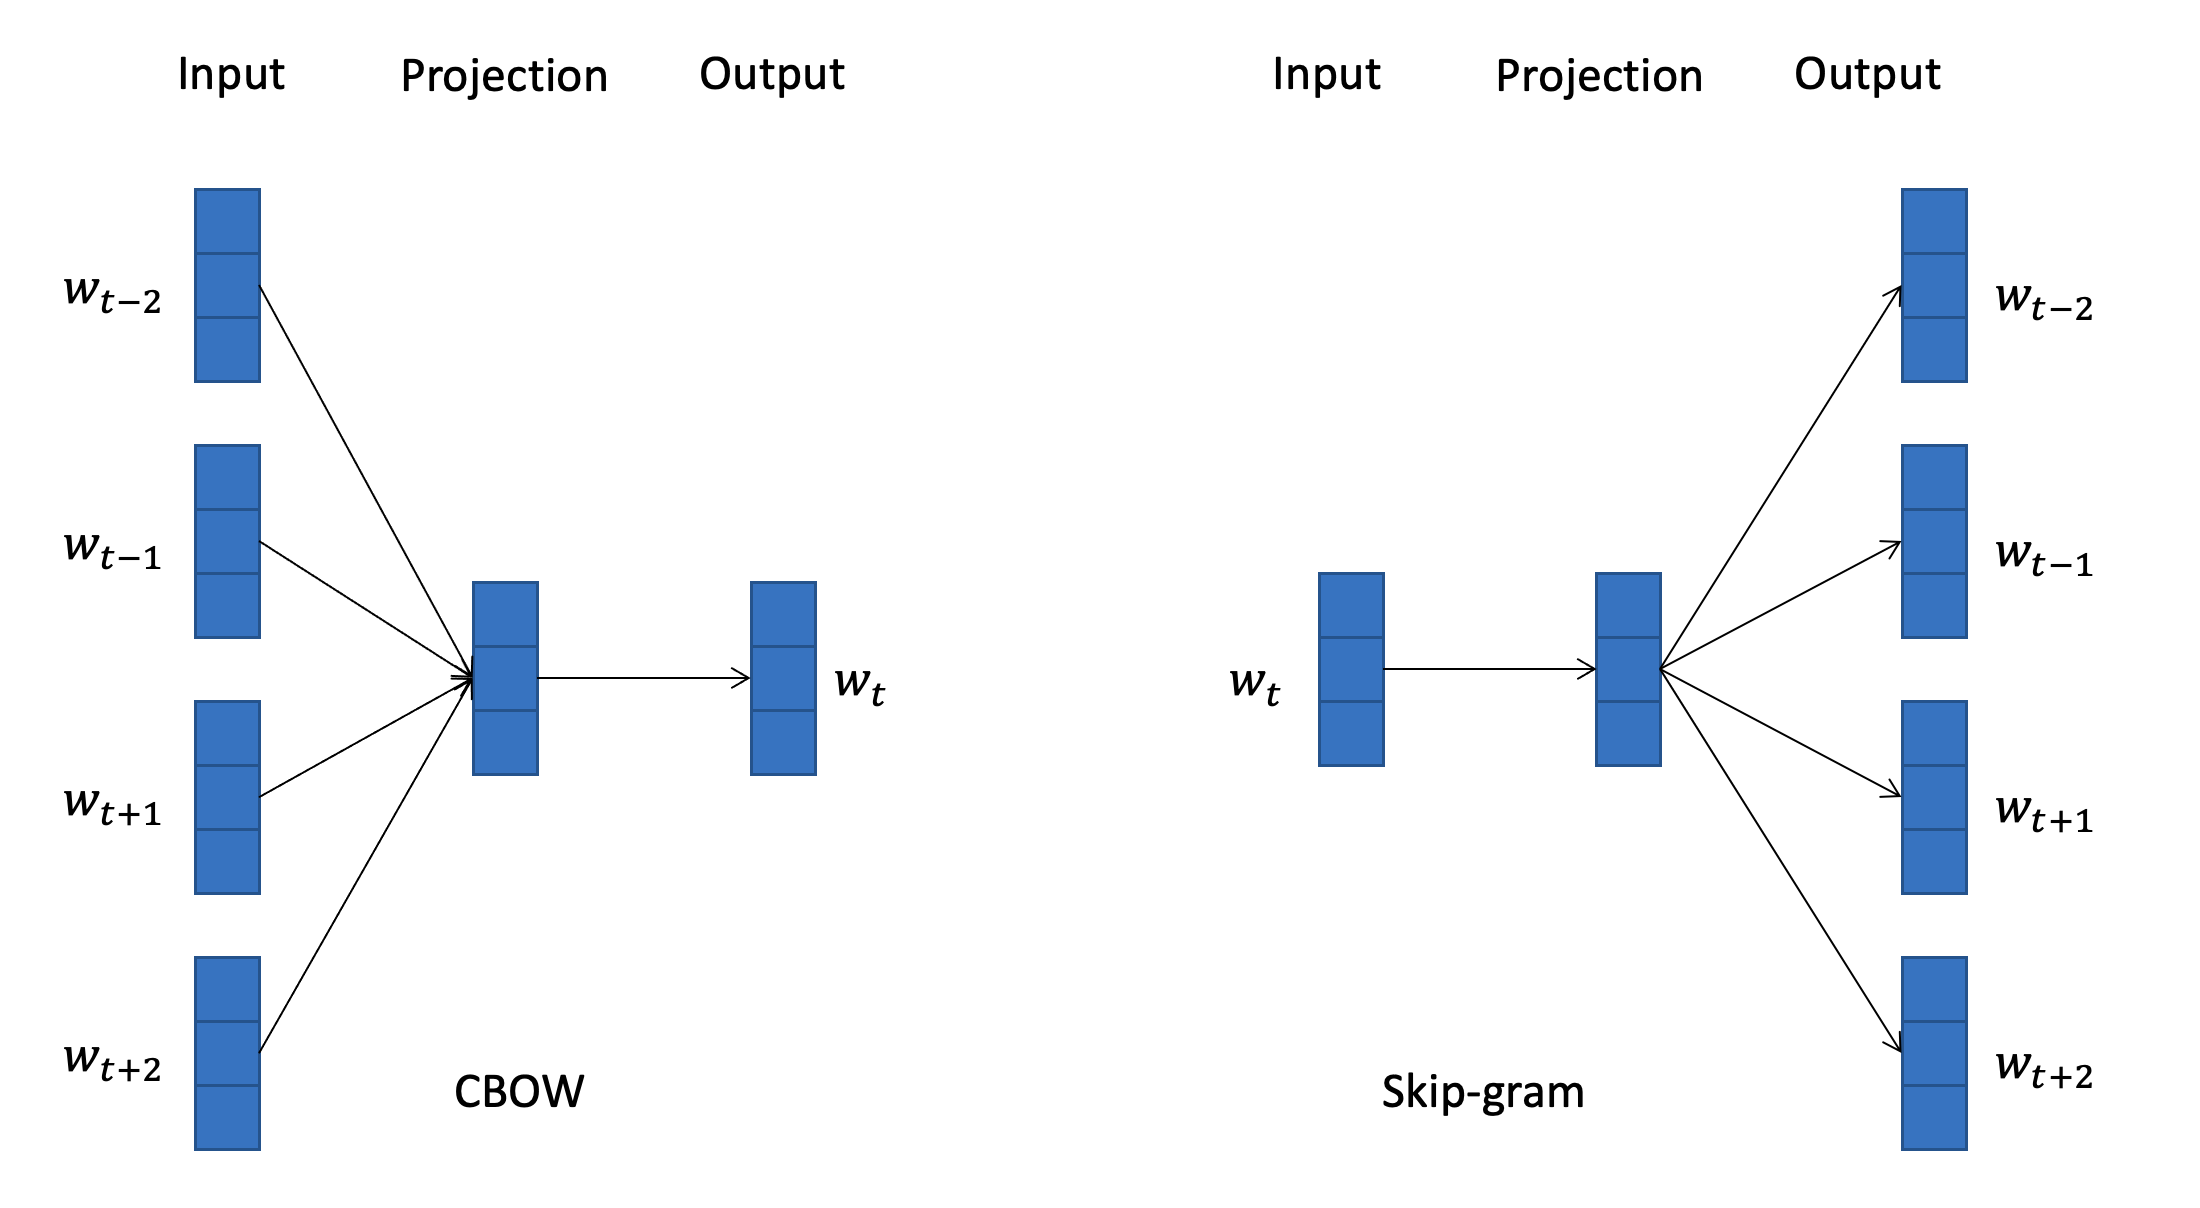
\includegraphics[width=1.0\textwidth]{ch2-fig4.png}
	\caption{Multi−head Attention}
	\label{fig4}
\end{figure}
$$\vec{x}_{i}^{\prime}=\|_{k=1}^{K} \sigma\left(\sum_{j \in \mathcal{N}_{i}} \alpha_{i j}^{k} \mathbf{W}^{k} \vec{x}_{j}\right)$$
K-averaging is used to replace the join operation and to delay the application of the final nonlinear function. The attention coefficients between different nodes after regularization are obtained by the above operation and can be used to predict the output characteristics of each node:
$$\vec{x}_{i}^{\prime}=\sigma\left(\frac{1}{K} \sum_{k=1}^{K} \sum_{j \in \mathcal{N}_{i}} \alpha_{i j}^{k} \mathbf{W}^{k} \vec{x}_{j}\right)$$
There are a total of $K$ attention mechanisms to consider, with $k$ denoting the kth of $K$. 

%GAT获取的questions,knowledge point和answer的嵌入。分别记作$\mathbf{E}_{p} \in \mathbb{R}^{|\mathcal{P}| \times d}$,$ \mathbf{E}_{q} \in \mathbb{R}^{|\mathcal{Q}| \times d}$, $\mathbf{E}_{a} \in \mathbb{R}^{2 \times d}$,用z代表embedding size。

From this layer, we got the embedded question and knowledge point vector $\hat{q}_{i} =  \vec{x}_{i}^{\prime}$, which would be passed into the Transformer Block in Knowledge tracing module.

\subsection{Transformer-based knowledge tracing}

The input of transformer Block is the concatenation of the embedded question $\hat{q}_{i}$ and corresponding answer $a_i$, i.e. $e_i=\hat{q}_{i}\|a_i$. The general structure is like Figure \ref{fig5} and the Transformer-block is like Figure \ref{fig6}. The traditional Transformer model is modified to apply to knowledge tracing task. The Transformer can learn the W-matrix relating underlying knowledge points and questions rather than directly learn the representation of each question. This allows the model to learn deeper connections between problems, resulting in better inference performance. It can cluster problems with similar knowledge points and reduce the variance for less frequent problems.
\begin{figure}[h]
	\centering
	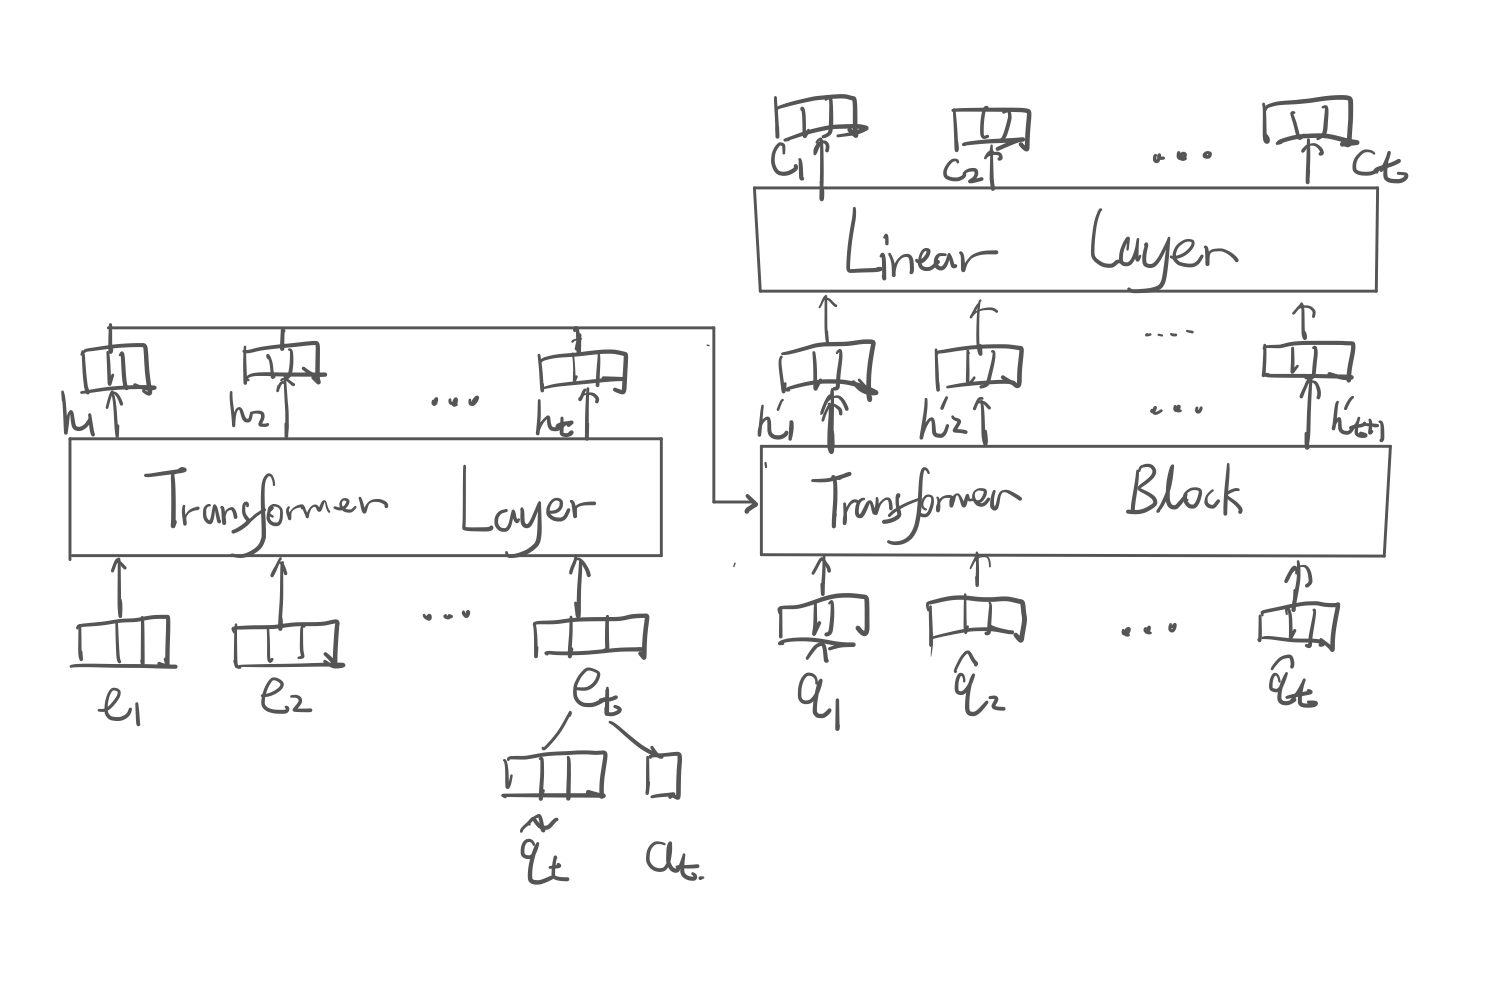
\includegraphics[width=1.0\textwidth]{ch2-fig5.jpeg}
	\caption{The Transformer architecture}
	\label{fig5}
\end{figure}

\begin{figure}[h]
	\centering
	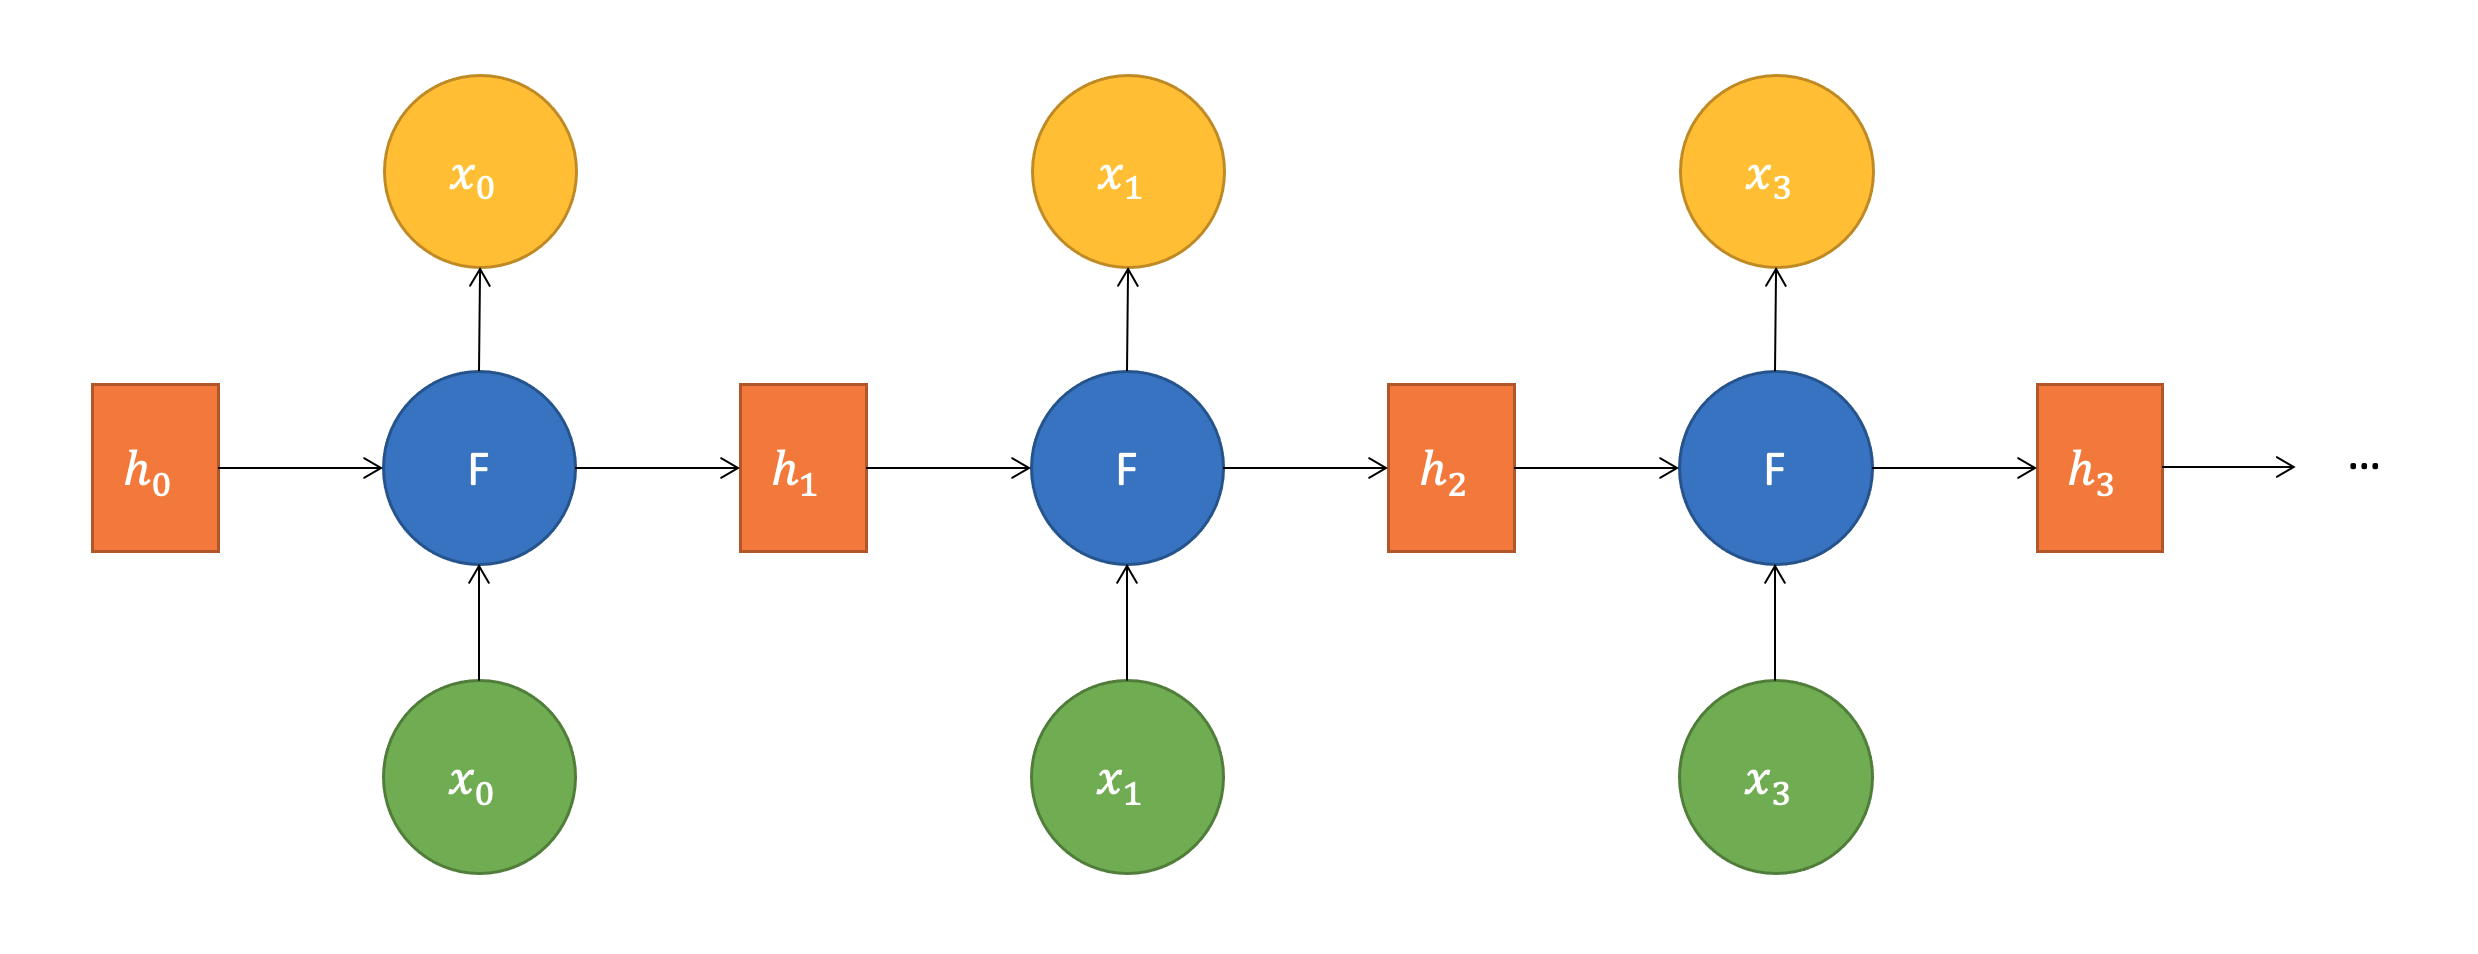
\includegraphics[width=0.5\textwidth]{ch2-fig6.png}
	\caption{The Transformer-block architecture}
	\label{fig6}
\end{figure}

The output of Embedding layer $e_i$ is passed into a Transformer Block, which is a self-attention module. 
$$
\begin{array}{c}
q_{i}=Q e_{i}, k_{i}=K e_{i}, v_{i}=V e_{i} \\
A_{i j}=\frac{q_{i} k_{j}+b\left(\Delta t_{i-j}\right)}{\sqrt{d_{k}}}, \forall j \leq i \\
h_{i}=\sum_{j \leq i} \operatorname{softmax}\left(A_{i j}\right) v_{j}
\end{array}
$$

the masked attention layer first extracts query gi, key k;, and value y; from the inputs ei. It then assign an attention, Aii, to a past interaction e, based on two components: 
\begin{enumerate}
  \item $q_i k_j$, the query-key agreement between $e_i$ and $e_j$, which could be interpreted as the degree of latent skills overlapping between interaction $e_i$ and $e_j$;
  \item A time gap bias, $b(\delta t_{i-j})$, which adjusts the attention weight by the time gap between interactions $e_i$ and $e_j$. The hidden representation $h_i$ is a weighted sum of the past value representations of $e_i$.
\end{enumerate}

A Transformer block also have feedforward layer, normalization layer, and residual connections. The outputs of a stack of Transformer blocks is feed to the linear layer before calculating the final loss. $e_{i+1}$ and $e_{i+1}^*$ are the results of applying Interaction Mapping Layer to $(\hat{q}_{i+1}, 1)$ and $(\hat{q}_{i+1}, 0)$.

$$
\begin{array}{c}
p_{i+1}=\frac{\exp \left(h_{i} e_{i+1}\right)}{\exp \left(h_{i} e_{i+1}\right)+\exp \left(h_{i} e_{i+1}^{*}\right)} \\
\text { Loss }=-\sum_{i} c_{i+1} \log \left(p_{i+1}\right)+\left(1-c_{i+1}\right) \log \left(1-p_{i+1}\right)
\end{array}
$$

\subsection{The Knowledge State }
\mynote{TODO}

\section{Experiments}
In this section, we conduct several experiments to investigate the performance of our model. We first evaluate the prediction error by comparing our model with other baselines on three public datasets. Then the paper make ablation studies on the GAT and GATKT to show their effectivenes. Finally, the paper evaluates the design decisions of the recap module to investigate which design performs better.
\subsection{Datasets}
To evaluate our model, the experiments are conducted on three widely-used datasets in KT and the detailed statistics are shown in Table \ref{ch2-tb1}.
\begin{itemize}
  \item ASSIST09 was collected during the school year 2009-2010 from ASSIST ments online education platform. We conduct our experiments on" skill- builder " dataset. Following the previous work 32, we remove the duplicated records and scaffolding problems from the original dataset. This dataset has 3852 students with 123 skills, 17, 737 questions and 282,619 exercises
  \item ASSIST12 was collected from the same platform as ASSIST09 during the school year 2012-2013. In this dataset, each question is only related to one skill, but one skill still corresponds to several questions. After the same data processing as ASSIST09, it has 2, 709, 436 exercises with 27, 485 students, 265 skills and 53, 065 questions.
  \item Ednet was collected by 51. As the whole dataset is too large, we randomly select 5000 students with 189 skills, 12, 161 questions and 676, 974 exercises
\end{itemize}
 
\begin{table}[h]
  \centering
  \caption{Dataset Statistics}
  \label{ch2-tb1}
  \begin{array}{cccc}
    \hline & \text { ASSIST09 } & \text { ASSIST12 } & \text { EdNet } \\
    \hline \text { #students } & 3,852 & 27,485 & 5000 \\
    \text { #questions } & 17,737 & 53,065 & 12,161 \\
    \text { #skills } & 123 & 265 & 189 \\
    \text { #exercises } & 282,619 & 2,709,436 & 676,974 \\
    \text { questions per skill } & 173 & 200 & 147 \\
    \text { skills per question } & 1.197 & 1.000 & 2.280 \\
    \text { attempts per question } & 16 & 51 & 56 \\
    \text { attempts per skill } & 2,743 & 10,224 & 8,420 \\
    \hline
    \end{array}
\end{table}

Note that for each dataset we only use the sequences of which the length is longer than 3 in the experiments as the too short sequences are meaningless. For each dataset, we split 80\% of all the sequences as the training set, 20\% as the test set. To evaluate the results on these datasets, we use the area under the curve (AUC)as the evaluation metric. 

\subsection{Baselines}
In order to evaluate the effeciveness of our proposed model, we use the following models as our baselines. 
\begin{itemize}
  \item BKT uses Bayesian inference for prediction, which models the knowledge state of the skill as a binary variable.
  \item DKT is the first method that uses deep learning to model knowledge tracing task. It uses recurrent neural network to model knowledge state of students
  \item DKVMN uses memory network to store knowledge state of different concepts respectively instead of using a single hidden state
  \item DKT-Q is a variant of DKT that we change the input of DKT from skills to questions so that the DKT model directly uses question information for prediction 
  \item DKIT-QS is a variant of DKT that we change the input of DKT to the concatenation of questions and skills so that the DKT model uses question and skill information simultaneously for prediction
\end{itemize}
  


\subsection{Performance}
Table \ref{ch2-tb2} reports the AUC results of all the compared methods. From the re sults we observe that our GATKT model achieves the highest performance over three datasets, which verifies the effectiveness of our model. To be specific, our proposed model GATKT achieves at least 1\% higher results than other baselines Among the baseline models, traditional machine learning models like BKT and KTM perform worse than deep learning models, which shows the effectiveness of deep learning methods. DKVMN performs slightly worse than DKT on average as building states for each concept may lose the relation information between concepts. On the other hand, we find that directly using questions as input may achieve superior performance than using skills. For the question-level model DKT-Q, it has comparable or better performance than DKT over ASSIST12 and Ednet datasets. However, DKT-Q performs worse than DKT in ASSIST09 dataset. The reason may be that the average number of attempts per question in ASSIS'T09 dataset is significantly less than other two datasets as observed in Table 1, which illustrates DKT-Q suffers from data sparsity problem. Besides, the AUC results of the model DKT-QS are higher than DKT-Q and DKT, except on ASSIST12 as it is a single-skill dataset, which indicates that considering question and skill information together improves overall performance.

\begin{table}[h]
	\centering
	\caption{AUC results over three datasets}
	\label{ch2-tb2}
	\begin{tabular}{cccc}
		\hline Model & ASSIST09 & ASSIST12 & EdNet \\
		\hline BKT & 0.6571 & 0.6204 & 0.6027 \\
		KTM & 0.7169 & 0.6788 & 0.6888 \\
		DKVMN & 0.7550 & 0.7283 & 0.6967 \\
		DKT & 0.7561 & 0.7286 & 0.6822 \\
		\hline DKT-Q & 0.7328 & 0.7621 & 0.7285 \\
		DKT-QS & 0.7715 & 0.7582 & 0.7428 \\
		\hline GATKT & $\mathbf{0 . 7 8 9 6}^{*}$ & $\mathbf{0 . 7 7 5 4}^{*}$ & $\mathbf{0 . 7 5 2 3}^{*}$ \\
		\hline	
	\end{tabular}
\end{table}



\section{Summary}
In this chapter, we propose a knowledge tracing model to employ high-order question-skill relation graphs into question and skill representations. Besides, to model the student's mastery for the question and related skills, we design a recap module to select relevant history states to represent student's ability. Then we extend a generalized interaction module to represent the student's mastery degree of the new question and related skills in a consistent way. 
